\subsection{Clustering}
\label{sec:clustering}

In general, clustering is an unsupervised approach used to group data points based on the similarity of their attributes. It is considered an exploratory activity as a part of data mining processes \citep{Fayyad_1996_IEEE}. After clustering, each cluster should have data whose attribute patterns are more similar among themselves than those of other clusters. \citet{Jain_1999_ACMCS} classifies clustering approaches in two categories: hierarchical and partitional. Aside from other technical details out of the scope of this paper, the basic difference between them is that hierarchical algorithms create nested partitions whereas partitional algorithms produce a single partition. 

We use a partitional, distance-based method known as \kmeans{}. \citet{Macqueen_1967_Proc} describes this method as a process for partitioning a $n$-dimensional population into $k$ sets on the basis of a sample. Its algorithm produces partitions that are reasonably efficient in the sense of within-class variance. It starts with a user defined number of clusters ($k$) and assigns a random mean value to each cluster (or randomly choose $k$ data-points and assigns them as cluster centers). After this, the algorithm computes the distances of all other data-points to the center of the cluster and uses the distance as a criteria to clustering the data points. Because the data resides in a multi-dimensional space (here defined by each metric), there are different ways of computing the distance of each data-point to the cluster's center. We use the Euclidean distance:
% 
\begin{equation}
	d(x_i, x_j) = \sqrt{ \sum_{k=1}^{n} \left( x_{i,k} - x_{j,k} \right)^2 } 
	\, ,
\end{equation}
% 
where $n$ is the number of features and $d$ is the distance of $x_i$ and $x_j$ in $n$-$dimensional$ domain. Once the distance is computed, the algorithms labels the data based on the proximity of each point to each cluster, computes the mean value of the data for each cluster, and updates the location of each cluster's center. \textcolor{red}{(How do we compute ``mean value'' and how do we recompute the ``center''? All what follows after this in the original text is too descriptive, and not specific enough. We need to go to the point and this is going in long description circles.)} 

{\color{gray}
	The algorithm repeats the steps unless the amount of updates among the cluster centers is less than a tolerance value.  \kmeans{} clustering has been applied in different applications, however, there is no clustering technique that is universally applicable in uncovering the variety of structures present in multidimensional datasets. Therefore, clustering is a subjective process. The same set of data items often needs to be partitioned differently for different application. In result, it is essential for the user of a clustering algorithm to not only have a thorough understanding of the particular technique being utilized, but also to know the details of the data gathering process and to have some domain expertise; the more information the user has about the data at hand, the more likely the algorithm would be able to succeed in assessing its true class structure. Domain concept can play several roles in the clustering process, and a variety of choices are available to the practitioner \citep{Jain_1999_ACMCS}. 

	The major problem with \kmeans{} algorithm is that it is sensitive to the selection of the initial partition and may converge to a local minimum of the criterion function value if the initial partition is not properly chosen. Another problem accompanying the use of \kmeans{} algorithm is the choice of the number of desired output clusters. Several variant of the \kmeans{} algorithm have been reported in the literature. Some of them attempt to select a good initial partition so that the algorithm is more likely to find the global minimum value, another variation is to permit splitting and merging of the resulting clusters \citep{Jain_1999_ACMCS}. 

	In our application the number of clusters is not a problem and there is a consensus among researchers in the number of clusters (i.e., poor, fair, good, excellent), however, our initial attempts represent that the results are highly sensitive to the initial clusters' center. 

	Every clustering algorithm uses some type of knowledge either implicitly or explicitly. In this study the background knowledge is a series of hypothetical stations. We assume that there are four stations with score of 3, 5, 7, and 9 for all of their metrics. Based on the score limits in section.~\ref{validation_metrics} we know these stations belong to poor, fair, good, and excellent classes, respectively. These background knowledge could help the clustering processing to be in right direction regarding the fact that increasing dimension of data could increase noise in clustering and cause difficulty to better partitioning. \citet{Wagstaff_2001_Proc}  demonstrated a modification of \kmeans{} clustering algorithm which uses the background information of the domain or dataset. The algorithm adds two types of constraints to the clustering including:
	% 
	\begin{itemize}
	\item{Must-link: constraints specify that two instances have to be in the same cluster.}
	\item{Cannot-link: constraints specify that two instance must not be placed in the same cluster.}
	\end{itemize} 
	% 
	The algorithm is described in detail in \citet{Wagstaff_2001_Proc}, however, in simple words, in the ordinary \kmeans{} process before assigning data to the closes cluster, it controls the must-link and cannot-link conditions. Therefore, in this case, the closest cluster's center is not necessarily the final cluster of the data. Fig.~\ref{fig:con_kmeans} presents the difference between ordinary and constrained k-means clustering approach using 4 points and 4 cluster centers. Fig.~\ref{fig:con_kmeans}.a presents the \kmeans{} without constrained. According to the definition and the explanation in this section, the closest cluster center for each points will get the points.
	
	Fig.~\ref{fig:con_kmeans}.b represents the constrained \kmeans{} approach, where, the closest cluster center is not necessarily the final cluster. The data points can not be in the same cluster, in result,  we assign them to different clusters in this case to satisfy the Cannot-link criteria. The best configuration happens when we minimize the distance between cluster centers and points. Using this method at each step the algorithm redistribute the 4 hypothetical stations to satisfy the cannot-link constraint. The visual inspection of the figures also confirms the accuracy of the method. Doing this, in the next iteration this data manipulation leads the cluster center in a direction to have the hypothetical station in the cluster and loose those data that is in far other side direction of the hypothetical station. Therefore, the cluster tend to have all data that similar to the hypothetical station. \\
	The end product of the clustering process is groups of data. Analysis of these groups, individually, gives the idea about the clusters in terms of within class variation. In these analysis we mainly study the behavior of different features in each cluster and isolate only the most descriptive features to be used in the supervised classifier that assumes a given number of classes in the data set. In the next section we provide a basics of decision tree algorithm. 

}

\begin{figure}
	\centering
	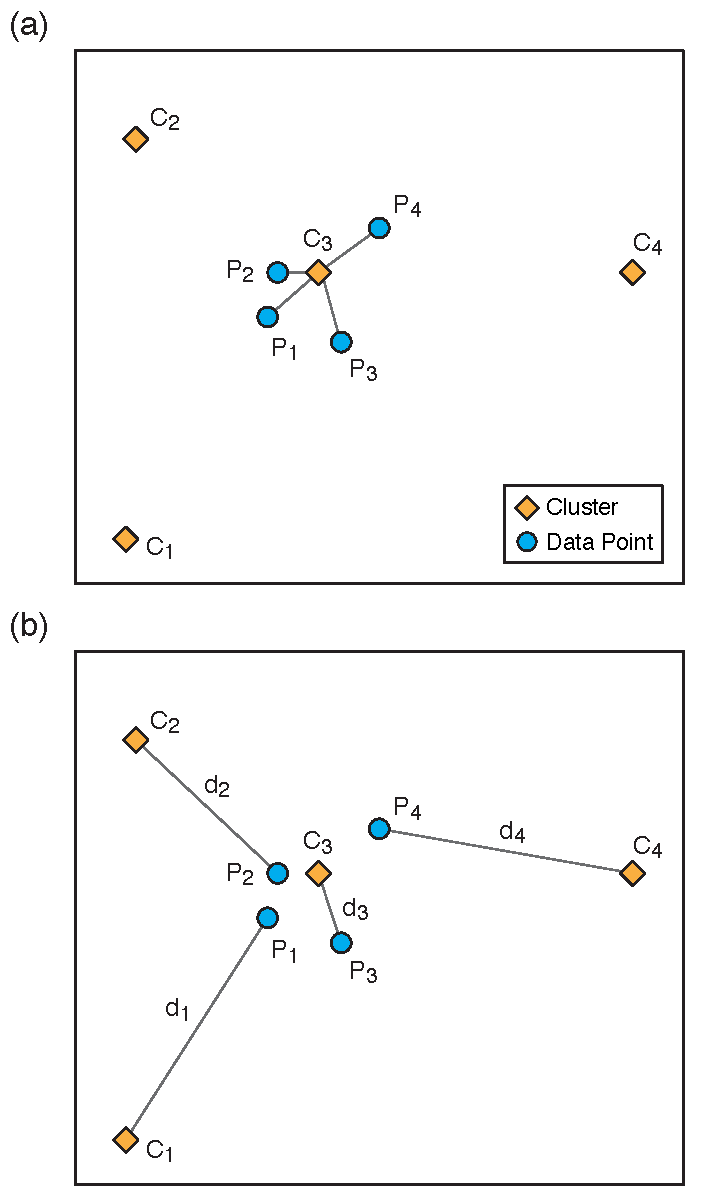
\includegraphics[width=\columnwidth]{figures/pdf/figure-04}
	\caption{Representation of the (a) ordinary, and (b) constrained \kmeans{} approaches for four data-points (P) and four cluster centers (C) in a 2D dataset space, where all the data-points are constrained to be cannot-link points. }
	\label{fig:con_kmeans}
\end{figure}

% In other words, the points cannot be in the same cluster. In the constrained \kmeans{} approach we redistribute the points such that the $\sum{d}$ becomes minimum.

% ===========================================================================================
%
% OLD NAEEM VERSION
% 
% Clustering is an unsupervised approach for grouping of data based on measure of similarity and it is considered as an exploratory activity as a part of data mining process \citep{Fayyad_1996_IEEE}. In each valid cluster, patterns are more similar in each other than they are to pattern belonging to a different cluster. Many clustering algorithms are developed for different application, however, study the difference of them is beyond the scope of this paper. In general, at the top level,  \citet{Jain_1999} distinguished the clustering approach into Hierarchical and Partitional approaches. Aside from differences in application and technical details in implementation, hierarchical methods produce nested series of partitions, while partitional methods produce only one. In this study we are interested in using partitional, distance based clustering algorithm, which is also known as \kmeans{} algorithm.  \citet{Macqueen_1967_Proc}  described a process for partitioning an $n$-$dimensional$ population into $k$ sets on the basis of a sample. The process appears to give partitions which are reasonably efficient in the sense of within-class variance. For numerical values, \kmeans{} algorithm starts with a user defined number of clusters (k) and assign a random mean value for each cluster (or randomly choose k data and assign them as cluster centers.) Then it computes the distance of data and cluster centers. A variety of distance measures are in use in different studies, however, we use the Euclidean distance through 

% \begin{equation}
% d(x_i,x_j)=\sqrt{\Sigma_{k=1}^{n}(x_{i,k} - x_{j,k})^2},
% \end{equation}

% where $n$ is the number of features and $d$ is the distance of $x_i$ and $x_j$ in $n$-$dimensional$ domain. After computing the distance of the points from each clusters' mean (center), the algorithm continues with labeling the data after the closest cluster. At the next iteration, it computes the mean value of data for each cluster and updates the clusters' centers. The algorithm repeats the steps unless the amount of updates among the cluster centers is less than a tolerance value.  \kmeans{} clustering has been applied in different applications, however, there is no clustering technique that is universally applicable in uncovering the variety of structures present in multidimensional datasets. Therefore, clustering is a subjective process. The same set of data items often needs to be partitioned differently for different application. In result, it is essential for the user of a clustering algorithm to not only have a thorough understanding of the particular technique being utilized, but also to know the details of the data gathering process and to have some domain expertise; the more information the user has about the data at hand, the more likely the algorithm would be able to succeed in assessing its true class structure. Domain concept can play several roles in the clustering process, and a variety of choices are available to the practitioner \citep{Jain_1999}. 

% The major problem with \kmeans{} algorithm is that it is sensitive to the selection of the initial partition and may converge to a local minimum of the criterion function value if the initial partition is not properly chosen. Another problem accompanying the use of \kmeans{} algorithm is the choice of the number of desired output clusters. Several variant of the \kmeans{} algorithm have been reported in the literature. Some of them attempt to select a good initial partition so that the algorithm is more likely to find the global minimum value, another variation is to permit splitting and merging of the resulting clusters \citep{Jain_1999}. 

% In our application the number of clusters is not a problem and there is a consensus among researchers in the number of clusters (i.e., poor, fair, good, excellent), however, our initial attempts represent that the results are highly sensitive to the initial clusters' center. 

% Every clustering algorithm uses some type of knowledge either implicitly or explicitly. In this study the background knowledge is a series of hypothetical stations. We assume that there are four stations with score of 3, 5, 7, and 9 for all of their metrics. Based on the score limits in section.~\ref{validation_metrics} we know these stations belong to poor, fair, good, and excellent classes, respectively. These background knowledge could help the clustering processing to be in right direction regarding the fact that increasing dimension of data could increase noise in clustering and cause difficulty to better partitioning. \citet{Wagstaff_2001_Proc}  demonstrated a modification of \kmeans{} clustering algorithm which uses the background information of the domain or dataset. The algorithm adds two types of constraints to the clustering including:\\
% \begin{itemize}
% \item{Must-link: constraints specify that two instances have to be in the same cluster.}
% \item{Cannot-link: constraints specify that two instance must not be placed in the same cluster.}
% \end{itemize} 
% The algorithm is described in detail in \citet{Wagstaff_2001_Proc}, however, in simple words, in the ordinary \kmeans{} process before assigning data to the closes cluster, it controls the must-link and cannot-link conditions. Therefore, in this case, the closest cluster's center is not necessarily the final cluster of the data. Fig.~\ref{fig:con_kmeans} presents the difference between ordinary and constrained k-means clustering approach using 4 points and 4 cluster centers. Fig.~\ref{fig:con_kmeans}.a presents the \kmeans{} without constrained. According to the definition and the explanation in this section, the closest cluster center for each points will get the points.
% Fig.~\ref{fig:con_kmeans}.b represents the constrained \kmeans{} approach, where, the closest cluster center is not necessarily the final cluster. The data points can not be in the same cluster, in result,  we assign them to different clusters in this case to satisfy the Cannot-link criteria. The best configuration happens when we minimize the distance between cluster centers and points. Using this method at each step the algorithm redistribute the 4 hypothetical stations to satisfy the cannot-link constraint. The visual inspection of the figures also confirms the accuracy of the method. Doing this, in the next iteration this data manipulation leads the cluster center in a direction to have the hypothetical station in the cluster and loose those data that is in far other side direction of the hypothetical station. Therefore, the cluster tend to have all data that similar to the hypothetical station. \\
% The end product of the clustering process is groups of data. Analysis of these groups, individually, gives the idea about the clusters in terms of within class variation. In these analysis we mainly study the behavior of different features in each cluster and isolate only the most descriptive features to be used in the supervised classifier that assumes a given number of classes in the data set. In the next section we provide a basics of decision tree algorithm. 


% \begin{figure}
%     \centering
%     \includegraphics
%       %  [width=\columnwidth]
%         [width=200px]
%         {figures/pdf/Figure_4.pdf}
%     \caption{ Representation of ordinary (a) and constrained (b) \kmeans{} approach. There are four data points (p) and four cluster centers (c) as a sample of $2$-$Dimensional$ dataset. All points are defined as cannot-link constraints. In other words, the points cannot be in the same cluster. In the constrained \kmeans{} approach we redistribute the points such that the $\sum{d}$ becomes minimum.}
%     \label{fig:con_kmeans}
% \end{figure}

